\documentclass[cjk]{beamer}
\usetheme{UIBK} %Standard UIBK Template
\usefonttheme[onlymath]{serif}

\usepackage[utf8]{inputenc}
\usepackage{tikz}
\usepackage{listings}
\definecolor{mygreen}{rgb}{0,0.6,0}
\definecolor{mygray}{rgb}{0.5,0.5,0.5}
\definecolor{mymauve}{rgb}{0.58,0,0.82}
\definecolor{bggray}{rgb}{0.93,0.95,0.94}

\lstset{ %
backgroundcolor=\color{bggray},      % choose the background color
columns=fullflexible,
tabsize=4,
breaklines=true,               % automatic line breaking only at whitespace
captionpos=b,                  % sets the caption-position to bottom
commentstyle=\color{mygreen},  % comment style
escapeinside={\%*}{*)},        % if you want to add LaTeX within your code
keywordstyle=\color{blue},     % keyword style
stringstyle=\color{mymauve}\ttfamily,  % string literal style
frame=shadowbox,
rulesepcolor=\color{red!20!green!20!blue!20},
% identifierstyle=\color{red},
language=c++,
numbers=left,
numberstyle=\tiny\sffamily,
basicstyle=\tiny\ttfamily,% size of fonts used for the code
escapeinside=``,
xleftmargin=0.6em,
xrightmargin=0.6em,
aboveskip=1em
}
\usepackage{fontenc}
\usepackage[]{xeCJK,fontspec}
\setCJKmainfont{FandolSong}%{SimSun}
\setmainfont{CMU Serif}
\setsansfont{CMU Sans Serif}
\setmonofont{Sarasa Fixed SC}
%\setCJKmainfont{叶根友疾风劲草}
\setCJKfamilyfont{song}{FandolSong}
\newcommand{\song}{\CJKfamily{song}}
\setCJKfamilyfont{kaiti}{FandolKai}
\newcommand{\kaiti}{\CJKfamily{kaiti}}
\setCJKfamilyfont{heiti}{FandolHei}
\newcommand{\heiti}{\CJKfamily{heiti}}
%\usefonttheme[onlymath]{serif}
\usepackage{indentfirst}

\usepackage{graphics,tcolorbox}
\usepackage{graphicx,xcolor,xcolor-solarized}
\usepackage{amsmath,amssymb,amsfonts}
%\usepackage{manfnt}
\newcommand{\chuhao}{\fontsize{42pt}{\baselineskip}\selectfont}

\mode<article> % 仅应用于article版本
{
  \usepackage{beamerbasearticle}
  \usepackage{fullpage}
  \usepackage{hyperref}
}

\usefoottemplate{\vbox{%
\tinycolouredline{structure!120}%
 {\color{white}\textbf{\insertshortauthor\hfil%
 \insertshorttitle}\hfil   \insertframenumber{} / \inserttotalframenumber}%\hfil
}}
\makeatother
\newtheorem{原因}{{原因}}[section]
\newtheorem{定义2.2}{{定义2.2}}[section]
\newtheorem{引理2.1}{{引理2.1}}[section]
\newtheorem{引理2.2}{{引理2.2}}[section]
\newtheorem{定理2.1}{{定理2.1}}[section]
\newtheorem{定理2.2}{{定理2.2}}[section]
\newtheorem{为什么追求高精度?}{{为什么追求高精度?}}[section]
%\newtheorem{definition}{{definition}}[section]
\newtheorem{lem}{{引理}}[section]
\newtheorem{remark}{{注记}}[section]
\newtheorem{dingyi}{{定义}}[section]
\renewcommand{\figurename}{图}
%\usepackage[default]{comfortaa}

\author{组员:仇琨元\ 徐嘉睿\ 肖锐卓\ 吴雨飞}
\title{Matrix Multiplication Acceleration}
\subtitle{Implemented By Strassen Algorithm and Intel(R) Math Kernel Library}
\institute{Insitute of EEE \\ SUSTech}
\date{\today}

\begin{document}

%titlepage without header/footer and framenumbering
\begin{frame}[plain]
  \titlepage
\end{frame}

\begin{frame}{Contents}
  \tableofcontents
\end{frame}


%show table of contents at the beginning of every section
\AtBeginSection[]{
  \begin{frame}<beamer>
    \frametitle{Contents}
    \tableofcontents[currentsection]
  \end{frame}
}

\section{Background}
\begin{frame}
  \frametitle{\textbf{Necessity of Matrix Multiplication Acceleration}}
  \vspace{5mm}
  \small
  ~~~~The multiplication of two matrices is one of the most basic operations of linear algebra and scientific computing.

  ~~~~Modern signal processing, artificial intelligence and computer vision are all based on the fast and accurate algorithm of matrix multiplication, LU/QR/SVD decomposition and many other operations.

\end{frame}
\begin{frame}
  \frametitle{\small\textbf{Comparison of the time costs of computing the FFT}}

  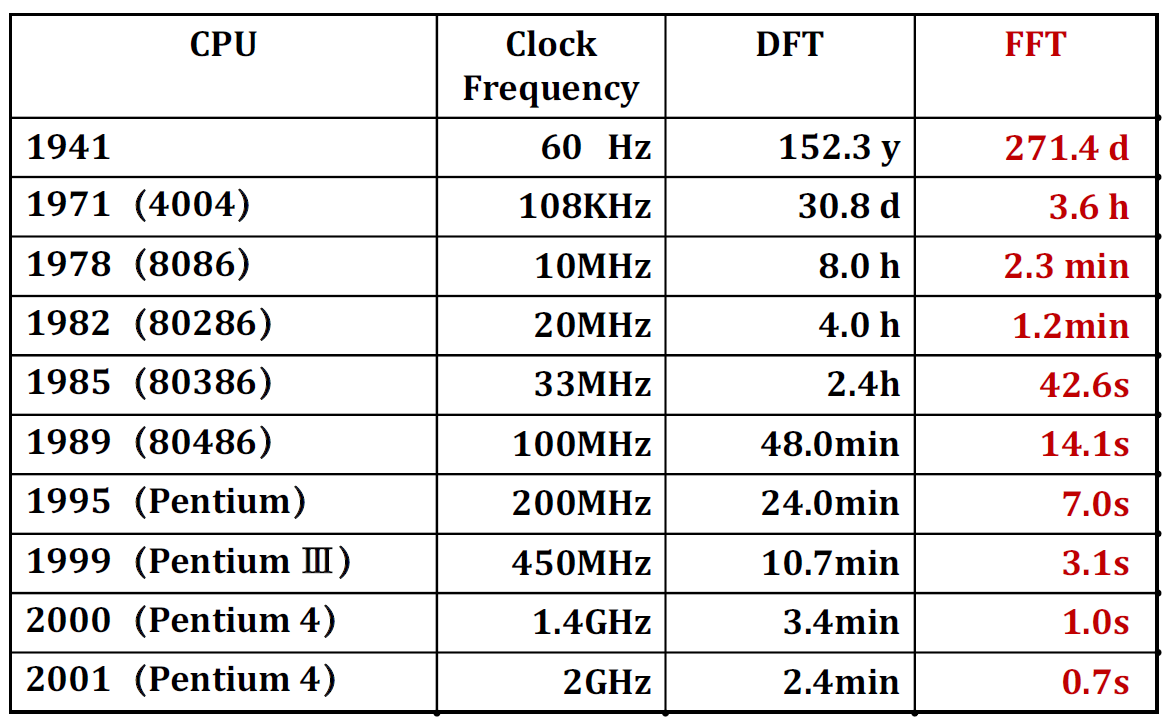
\includegraphics[height=5.0cm]{fftvel.png}

\end{frame}


\section{Therotical Analysis}
\subsection{Brute-Force Algorithm}
\begin{frame}[fragile]
  \frametitle{\textbf{Brute-Force Algorithm}}
  ~~~~The Strassen Multiplication uses divide-conquer to reduce the time complexity of MM operations.
  Normal MM uses 3 nested loops to perform the vector dotting and traversal of the rows and columns of the 2 operands:
  \begin{lstlisting}
    STANDARD-MATRIX-MULTIPLY (A,B):
    let C be a new m*n matrix
      for i <- 1 to m
        for j <- 1 to n
          C[i,j] = 0
            for k = 1 to p
                C[i,j] += A[i,k]*B[k,j]
      return C
  \end{lstlisting}
\end{frame}
\begin{frame}
  \frametitle{\textbf{Brute-Force Algorithm}}

  From the pseudocode above, let MUL, ADD, READ and WRITE refers the corresponding \(assembly\) commands of the computer.
  Each nested loop multiplies the time complexity by its iteration number:
  \begin{equation}
    \begin{aligned}
      T(\text{Naive})                  & =m\cdot n\cdot p\cdot (T(\text{\small MUL}+\text{\small ADD}+\text{\small READ}+\text{\small WRITE})) \\
                                       & =\Theta(mnp)                                                                                          \\
      m=n=p\Rightarrow T(\text{Naive}) & =\Theta(n^{3})
    \end{aligned}
  \end{equation}

\end{frame}
\subsection{Strassen Algorithm}
\begin{frame}[fragile]
  \frametitle{\textbf{Strassen Algorithm}}
  Pseudocode of the Strassen algorithm:
  \begin{lstlisting}
    STRASSEN (MatrixA,MatrixB)
        N=MatrixA.rows
      Let MatrixResult be a new N×N matrix
      if N==1
        MatrixResult=MatrixA*MatrixB
      else
         // DIVIDE: partitioning input Matrices into 4 submatrices each
           for i  <-  0  to  N/2
               for j  <-  0  to  N/2
                  A11[i][j]  <-  MatrixA[i][j]
                  A12[i][j]  <-  MatrixA[i][j + N/2]
                  A21[i][j]  <-  MatrixA[i + N/2][j]
                  A22[i][j]  <-  MatrixA[i + N/2][j + N/2]

                  B11[i][j]  <-  MatrixB[i][j]
                  B12[i][j]  <-  MatrixB[i][j + N/2]
                  B21[i][j]  <-  MatrixB[i + N/2][j]
                  B22[i][j]  <-  MatrixB[i + N/2][j + N/2]
  \end{lstlisting}
\end{frame}
\begin{frame}[fragile]
  \frametitle{Strassen Algorithm}
  \begin{lstlisting}
  // CONQUER: here we calculate P1...P7 matrices
      P1 <- STRASSEN(A11, B12-B22)          //P1=A11(B12-B22)
      P2 <- STRASSEN(A11+A12, B22)          //P2=(A11+A12)B22
      P3 <- STRASSEN(A21+A22, B11)          //P3=(A21+A22)B11
      P4 <- STRASSEN(A22, B21-B11)          //P4=A22(B21-B11)
      P5 <- STRASSEN(A11+A22, B11+B22)      //P5=(A11+A22)(B11+B22)
      P6 <- STRASSEN(A12-A22, B21+B22)      //P6=(A12-A22)(B21+B22)
      P7 <- STRASSEN(A11-A21, B11+B12)      //P7=(A11-A21)(B11+B12)

        // calculate the result submatrices
      C11  <-  P5 + P4 - P2 + P6
      C12  <-  P1 + P2
      C21  <-  P3 + P4
      C22  <-  P5 + P1 - P3 - P7

        // MERGE: put them together and make our resulting Matrix
      for i  <-  0  to  N/2
         for j  <-  0  to  N/2
           MatrixResult[i][j]              <-  C11[i][j]
           MatrixResult[i][j + N/2]        <-  C12[i][j]
           MatrixResult[i + N/2][j]        <-  C21[i][j]
           MatrixResult[i + N/2][j + N/2]  <-  C22[i][j]
      return MatrixResult
\end{lstlisting}
\end{frame}
\begin{frame}
  \frametitle{Strassen Algorithm}

  Use the recursion function to evaluate the time complexity of the algorithm.
  For \(n\geqslant 2\),
  \begin{equation}
    \begin{aligned}
      T(2n)                          & =7T(n)+\Theta(n^{2})              \\
      \log_{2} n=k\Rightarrow T(k+1) & =7T(k)+\Theta(2^{2k})             \\
      \Rightarrow T(n)               & =O(n^{\log_{2}7})                 \\
                                     & \approx O(n^{2.81})<\Theta(n^{3})
    \end{aligned}
  \end{equation}
  The \(n\) in this result is the number of the \(Operation\), which is in propotition of the order of the matrix:
  \begin{equation}
    t(n)=\alpha \text{Rows},\alpha\in(1,\infty)
  \end{equation}
\end{frame}

\section{Methodology}
\begin{frame}[fragile]
  \frametitle{Experimental Enviornments and Test Code}
  \begin{block}{Experimental Enviormnent}
    \small
    CPU:Intel(R) Core(TM) i7-9750HQ@3.85\~\ 4.05GHz\\
    RAM:32GB 2666MHz
  \end{block}
  \begin{lstlisting}
    /**TEST CODE**/
    #include <...>
    int main(int argc, char *argv[]) {
      int turns = 10, rows = 2, cols = 2, interm = 0;
      randinit();
      for (int i = 0; i <= turns; i++) {
        LARGE_INTEGER t1, t2, tc;
        QueryPerformanceFrequency(&tc);
        QueryPerformanceCounter(&t1);
        /**Generate Rows and Elements**/
        printf_s("%3d   ", rows);
        /**Function To Be Timed**/
        QueryPerformanceCounter(&t2);
        time = (double) (t2.QuadPart - t1.QuadPart) / (double) tc.QuadPart;
        printf_s("%.3f\n", time);
        }
      getchar();
      return 0;
    }
  \end{lstlisting}
\end{frame}


\section{Experiment Results}
\subsection{Native Implementation of Strassen Algorithm using C++}
\begin{frame}
  \frametitle{Naive Matrix Multiplication implemented using C++}

  By implementing naive MM and Strassn algorithm on C++ and fit the data, the standard data of the two algorithms are
  \begin{equation}
    \begin{aligned}
      T(N)   & =O(n^{3.371}) \\
      T(S;2) & =O(n^{3.546})
    \end{aligned}
  \end{equation}
  \begin{columns}
    \column{0.65\textwidth}
    \begin{figure}[htb]
      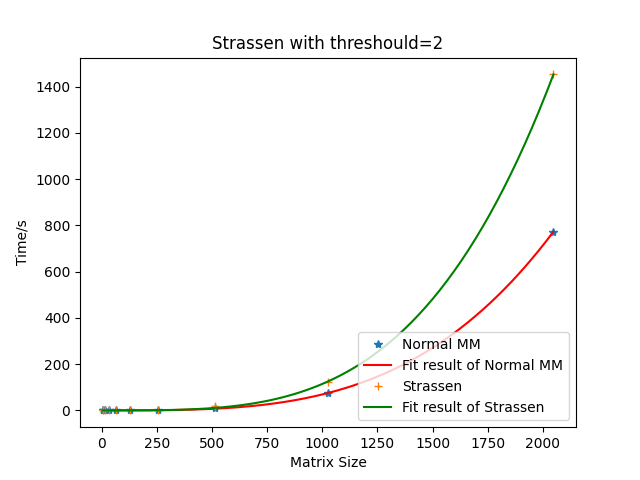
\includegraphics[width=0.8\linewidth]{th=2.png}
    \end{figure}
    \column{0.35\textwidth}
    This result shows that the Strassen Algorithm is seemingly faster than the brute-forcing MM, but neither of them even reaches the time complexity of \(O(n^3)\).
  \end{columns}
\end{frame}
\subsection{Strassen Algorithm with Minimun Size Threshold}
\begin{frame}
  \frametitle{Strassen Algorithm with Minimun Size Threshold}
  The main reason causing the Strassen Algorithm slower than the brute-forcing algorithm is the time costs in tracebacking the recursion.
  Thus, the time cost of the Strassen Algorithm can be significantly reduced by calibrating the crosspoint and setting the minimum size of
  recursion.
  \begin{equation}
    \begin{aligned}
      T(N)    & =O(n^{3.384}) \\
      T(S;32) & =O(n^{3.337})
    \end{aligned}
  \end{equation}
  And the constant of the Strassen Algorithm is about \(1/3\) of that of the brute-forcing algorithm.
\end{frame}
\begin{frame}
  \frametitle{Strassen Algorithm with Minimun Size Threshold}

  \begin{figure}[htb]
    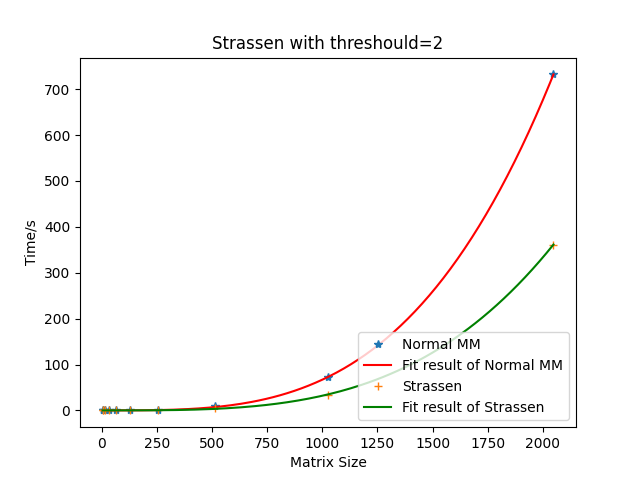
\includegraphics[width=0.9\linewidth]{th=64.png}
  \end{figure}

\end{frame}


\section{Hardware Optimization}
\subsection{Cache Alignement}
\begin{frame}[fragile]
  \frametitle{Acceleration of Brute-Force MM}

  To improve the performance of the brute-forcing MM, use a alternative order of multiplication:
  \begin{lstlisting}
    Alternative-Order-MM(Matrix A,Matrix B):
      for i in [0:length(A)]:
        for k in [0:length(A[0])]:
          s=A[i][k]
          for j in [0:length(B[0])]:
            Result[i][k]+=s*B[k][j]
          end
        end
      end
  \end{lstlisting}
  This inversion of the order in computing the matrix multiplication has the maximized accuracy when accessing the CPU cache, avoiding the interruption in the address sequence of the processor.
\end{frame}
\begin{frame}
  \frametitle{Strassen Algorithm with Improved Cache Accuracy}
  With the patch above, the Strassen algorithm can meet the therotical time complexity:
  \begin{equation}
    \begin{aligned}
      T(N)    & =O(n^{2.991}) \\
      T(S;32) & =O(n^{2.816})
    \end{aligned}
  \end{equation}
  \begin{columns}
    \column{0.6\textwidth}
    \begin{figure}[htb]
      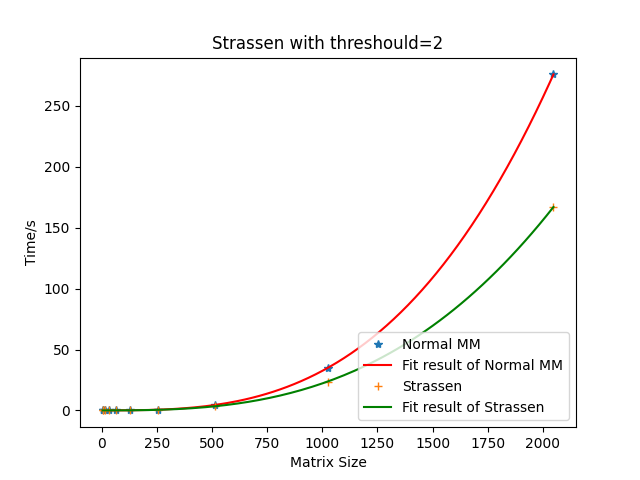
\includegraphics[width=0.8\linewidth]{th=32_ijk.png}
    \end{figure}
    \column{0.6\textwidth}
    \begin{figure}[htb]
      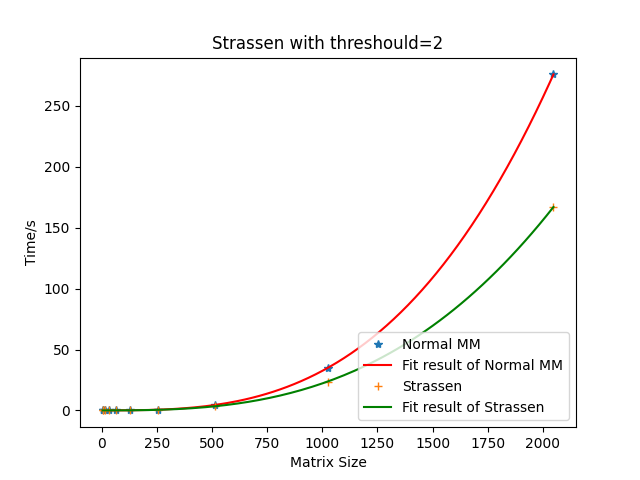
\includegraphics[width=0.8\linewidth]{th=64_ijk.png}
    \end{figure}
  \end{columns}
\end{frame}
\begin{frame}
  \frametitle{Sectioned Matrix Multiplication Algorithm}
  When the order of the matrix is very large, the length of the row-major array may exceed the maximum capacity of the L1 cache, the speed of the matrix multiplication will be limited. Let \(s\) be the sectioning number which the original matrix is divided by, and \(k\) be the polynomial degree of the time complexity, divide the matrix into small chunks so that the length of the chunks are below the maximum capacity of the L1 cache.
  \begin{equation}
    \begin{aligned}
      T(n;s)                                                        & =s^{k}t\left(\frac{n}{s}\right)^{k}                                                                         \\
      \frac{n}{k}<BW(\text{\scriptsize L1 Cache})\Rightarrow t(n/k) & =T(\text{\scriptsize PUSH})+T(\text{\scriptsize MUL})+T(\text{\scriptsize POP})                             \\
                                                                    & <<2T(\text{\scriptsize MOV})+T(\text{\scriptsize PUSH})+T(\text{\scriptsize MUL})+T(\text{\scriptsize POP})
    \end{aligned}
  \end{equation}
\end{frame}
\begin{frame}
  \frametitle{Sectioned Matrix Multiplication Algorithm}

  \begin{equation}
    \begin{aligned}
      T(N)   & =O(n^{3.013}) \\
      T(N;s) & =O(2.822)
    \end{aligned}
  \end{equation}
  \begin{figure}[htb]
    \begin{center}
      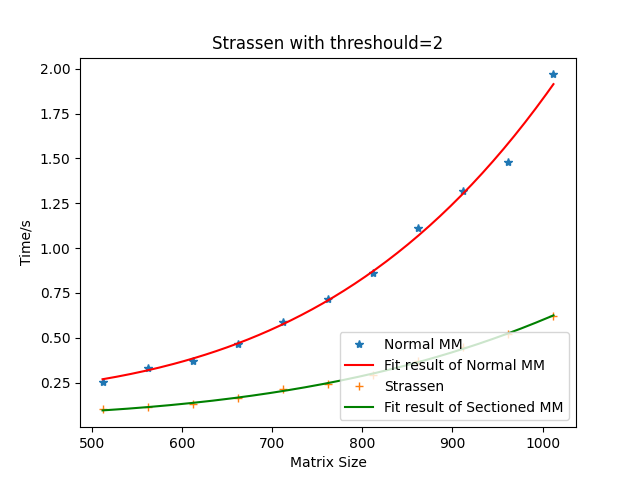
\includegraphics[height=5.0cm]{sub_naive.png}
    \end{center}
  \end{figure}
\end{frame}
\subsection{Intel MKL}
\begin{frame}
  \frametitle{Intel Math Kernel Library}

  \begin{figure}[htb]
    \begin{center}
      
\includegraphics[height=5.0cm]{yagao-logo.jpg}
    \end{center}
  \end{figure}

\end{frame}
\begin{frame}
  \frametitle{Intel Math Kernel Library}

  The \textbf{MKL} is a optimized implementation of many math functions exclusively on x86 architecture and processors supports the Intel SIMD instructions, especially in Intel(R) processors. This library is implemented by assembly codes and C++ codes that are extremely optimized by Intel SIMD instructions(\textbf{SSE},\textbf{AVX}), in order to maximize performance on matrix operations.
\end{frame}
\begin{frame}[fragile]
  \frametitle{C++ Test of double MM}

  \begin{lstlisting}
  int mkldgemm(int rowa, int cola, int colb) {
  using namespace std;
  double *A, *B, *C;
  int a = 1, b = 1;
  A = (double *) MKL_malloc(rowa * cola * sizeof(double), 64);
  B = (double *) MKL_malloc(cola * colb * sizeof(double), 64);
  C = (double *) MKL_malloc(rowa * colb * sizeof(double), 64);
  for (int i = 0; i < rowa * cola; ++i) {
      A[i] = randgen(-500, 500);
      }
  for (int i = 0; i < cola * colb; ++i) {
      B[i] = randgen(-500, 500);
      }
  for (int i = 0; i < rowa * colb; ++i) {
      C[i] = randgen(-650, 390) * randgen(-500, 500);
      }
  cblas_dgemm(CblasRowMajor, CblasNoTrans, CblasNoTrans,
    rowa, colb, cola, 1, A, cola,
    B, colb, b, C, colb);
  MKL_free(A);
  MKL_free(B);
  MKL_free(C);
  return 0;
  }
\end{lstlisting}

\end{frame}
\begin{frame}
  \frametitle{Performance of Intel MKL}
  Under the C++ implementation, The Intel MKL computes the 2500*2500 matrix multiplication within 6000 milliseconds, including filling the arrays.
  \begin{figure}[htb]
    \begin{center}
      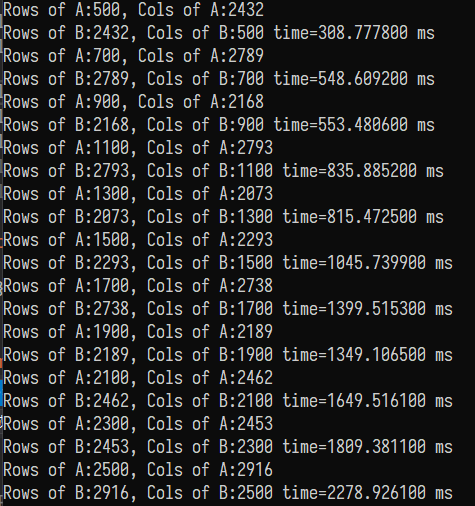
\includegraphics[height=4.2cm]{mkl_dgemm.png}
    \end{center}
  \end{figure}
\end{frame}
\begin{frame}
  \frametitle{Performance of Intel MKL}

  Under the Java implementation we adopted to accelerate the Strassen Algorithm, the deletion of the unnecessary array filling progress exploits the full capabilities of the MKL:
  \begin{equation}
    \begin{aligned}
      T(N)          & =4.008\times 10^{-9}n^{3.052}\approx \frac{1}{f_{\text{CPU}}}n^{3.052}     \\
      T(\text{MKL}) & =1.817\times 10^{-11}n^{2.982}\approx \frac{1}{250f_{\text{CPU}}}n^{2.982}
    \end{aligned}
  \end{equation}
  The extremely optimization based on the SIMD instructions of the Intel CPU made the MKL runs at 250x faster than the naive approach using merely sequential operations.
\end{frame}
\begin{frame}
  \frametitle{Performance of Intel MKL}

  \begin{figure}[htb]
    \begin{center}
      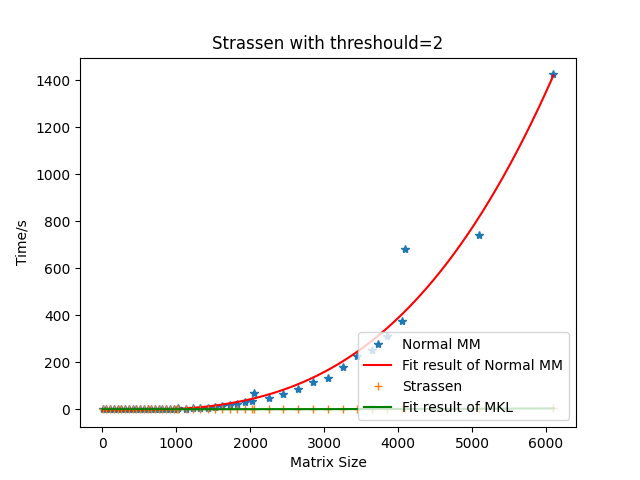
\includegraphics[height=5.0cm]{mkl.png}
    \end{center}
  \end{figure}

\end{frame}
\section{Acknowledgements}
\subsection{GitHub Site of the Project}
\begin{frame}
  \frametitle{Project Management via GitHub}



\end{frame}
%final slide
\begin{frame}[plain,noframenumbering]
  \begin{beamercolorbox}[wd=\paperwidth, ht=1.4cm,rounded=true,shadow=true]{final slide}
    \begin{center}
      {\huge Thank you for your attention!}
    \end{center}
  \end{beamercolorbox}
\end{frame}


\end{document}
